\chapter{Método para Avaliação de Classificadores Treinados na Base de Dados do Mercado Livre}
\label{cap-desenvolvimento}
Este capítulo expõe a metodologia utilizada para o desenvolvimento deste estudo, que visa classificar as perguntas de clientes reais de plataformas de \textit{e-commerce}, como o Mercado Livre, em relação ao atributo ao qual a pergunta se refere.

A Seção \ref{definicao_classes} retrata como foi feita a execução de requisições para a API do Mercado Livre com o objetivo de obter os atributos que aparecem no maior número de categorias de produtos. Além disso, mostra a definição dos atributos mais importantes e genéricos para se tornarem as classes.

A Seção \ref{coleta_dados} expõe o procedimento de importação de perguntas feitas por clientes reais do Mercado Livre através do banco de dados da GoBots. Além disso, são expostas a extração manual de mais perguntas de classes pouco presentes na base de dados e a criação manual de mais perguntas para que seja atingido um número mínimo de 15 perguntas por classe.

A Seção \ref{criacao_base_dados_rotulada} explica a criação e execução de um \textit{script Python} que coleta uma pergunta aleatória das que foram extraídas do banco de dados da GoBots e mostra para o usuário rotular manualmente, de forma iterativa.

A Seção \ref{pre_processamento_dados} descreve a definição das etapas de pré-processamento dos dados que foram executadas antes do treinamento dos algoritmos de classificação. Para o classificador BERTimbau, foi feita apenas a tokenização com o seu tokenizador. Para o classificador DIETClassifier, foram adicionadas outras etapas.

A Seção \ref{algoritmos_classificacao} apresenta o treinamento dos algoritmos de classificação, que foi baseado em diferentes configurações de pré-processamento dos dados, em diferentes hiperparâmetros de treino e em diferentes quantidades de classes. Além disso, a Seção \ref{algoritmos_classificacao} define o método para separação de dados em treino e teste.

A Seção \ref{medidas_metodo_avaliacao_classificadores} discorre sobre a criação de uma função responsável pelo cálculo das métricas acurácia, precisão, revocação e F1-score, bem como sobre a geração de matrizes de confusão. Além disso, a Seção \ref{medidas_metodo_avaliacao_classificadores} também explica como foi aplicada a ponderação sobre as métricas para conter o efeito do desbalanceamento das classes.

\section{Visão Geral do Método para Avaliação}

A Figura \ref{fig:etapas_desenvolvimento} apresenta as etapas de desenvolvimento deste estudo, que serão detalhadas nas próximas seções.

\begin{figure}[!ht]
    \centering
	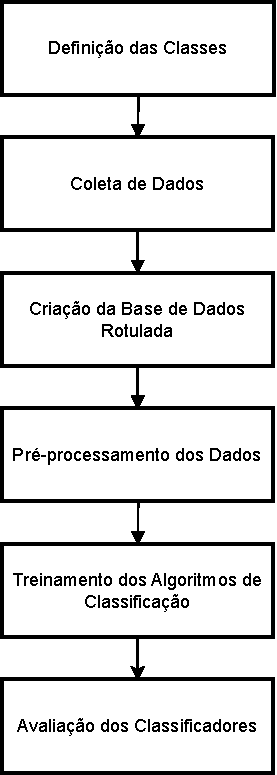
\includegraphics[width=0.25\linewidth]{metodologia_de_desenvolvimento2.pdf}
	\caption{Etapas do desenvolvimento deste estudo, que consiste em um método para avaliação de classificadores treinados na base de dados do Mercado Livre.}
	\label{fig:etapas_desenvolvimento}
\end{figure}

\section{Definição das Classes}
\label{definicao_classes}
Antes de coletar os dados que compuseram a base de dados, foi necessário definir quais atributos seriam considerados como classes. No Mercado Livre\footnote{\url{https://www.mercadolivre.com.br/}}, os produtos estavam organizados hierarquicamente em categorias. Essas categorias, por sua vez, estavam organizadas em um formato de Árvore de Categorias, que podia ser acessado com requisições via API\footnote{\url{https://developers.mercadolivre.com.br/pt_br/categorias-e-atributos}} usando o comando da Figura \ref{fig:comando_category_tree}.

\begin{figure}[htb]
    \centering
    \color{black}
    \begin{minted}{bash}
    $ curl https://api.mercadolibre.com/sites/MLB/categories/all > f.gz
    \end{minted}
    \caption{Comando para fazer \textit{download} de um arquivo compactado que possui a Árvore de Categorias completa do Mercado Livre brasileiro.}
    \label{fig:comando_category_tree}
\end{figure}

O Mercado Livre brasileiro possuía 32 categorias principais, e cada uma das categorias principais era dividida em dezenas de categorias secundárias, que por sua vez também podiam possuir outras subcategorias. Por exemplo, um carregador de celular era um produto que se encontrava em Celulares e Telefones > Acessórios para Celulares > Carregadores e Acessórios > Carregadores, de acordo com a estrutura proposta pelo Mercado Livre.

Como a GoBots fornece serviços para lojistas que vendem produtos das 11 categorias principais dispostas na Tabela \ref{table:categorias escolhidas}, essas foram as categorias de produtos escolhidas para compor a base de dados.

\begin{center}
\begin{table}[ht]
\caption{Categorias escolhidas para serem representadas na base de dados}
\label{table:categorias escolhidas}
\centering
    \begin{tabular}{|c|c|} 
     \hline
     \multicolumn{2}{|c|}{Categoria} \\
     \hline
     Acessórios para Veículos & Construção \\ 
     \hline
     Beleza e Cuidado Pessoal & Eletrodomésticos \\
     \hline
     Calçados, Roupas e Bolsas & Eletrônicos, Áudio e Vídeo \\
     \hline
     Câmeras e Acessórios & Esportes e Fitness\\
     \hline
     Casa, Móveis e Decoração & Ferramentas \\
     \hline
     Celulares e Telefones & \\
     \hline
    \end{tabular}
\end{table}
\end{center}

Para definir quais atributos serão considerados como classes, foi feito o \textit{download} da Árvore de Categorias usando o comando da Figura \ref{fig:comando_category_tree}. Em seguida, foi desenvolvido um código em \textit{Python} para percorrer essa Árvore de Categorias. Foram tomadas como base as categorias principais escolhidas e especificadas na Tabela \ref{table:categorias escolhidas}, e, após sucessivas iterações, juntou-se em uma lista todas as subcategorias dessas categorias principais, mantendo-se apenas as subcategorias que não possuem divisões.

Com a lista de todas as subcategorias desejadas disponível, novas requisições para a API do Mercado Livre foram feitas. Dessa vez, usando por milhares de vezes o comando da Figura \ref{fig:comando_category_attributes}, que retorna todos os atributos de uma determinada categoria. Com o auxílio de códigos em \textit{Python}, foram feitas transformações nesses dados: uma nova lista foi feita, descrevendo junto a cada subcategoria todos os seus possíveis atributos.

\begin{figure}[htb]
    \centering
    \color{black}
    \begin{minted}{bash}
    $ curl https://api.mercadolibre.com/categories/<id_cat>/attributes
    \end{minted}
    \caption{Comando para fazer \textit{download} de todos os atributos de uma determinada subcategoria do Mercado Livre brasileiro. \texttt{\textless id\_cat\textgreater} é um código único que identifica a subcategoria no conjunto de todas as categorias.}
    \label{fig:comando_category_attributes}
\end{figure}

Em seguida, foi criada uma nova lista com todos os atributos das subcategorias desejadas e o número de ocorrências em que esses atributos estão descritos nessas subcategorias. A Figura \ref{fig:top10_attributes} mostra os 10 atributos que mais aparecem nesse conjunto.

\begin{figure}[htb]
    \begin{lstlisting}[language=json,firstnumber=1]
    {
      "BRAND": 4892,
      "MODEL": 4892,
      "PACKAGE_HEIGHT": 4892,
      "PACKAGE_WIDTH": 4892,
      "PACKAGE_LENGTH": 4892,
      "PACKAGE_WEIGHT": 4892,
      "ITEM_CONDITION": 4892,
      "GTIN": 4890,
      "MPN": 4890,
      "SELLER_SKU": 4890,
      ...
    }
    \end{lstlisting}
    \caption{Os 10 atributos que são mais aceitos entre as subcategorias sem descendentes das categorias escolhidas e o número de subcategorias em que cada um aparece.}
    \label{fig:top10_attributes}
\end{figure}

Por último, foram escolhidos os atributos de maior interesse comercial da lista da Figura \ref{fig:top10_attributes} para serem as classes. O critério principal para a escolha foi selecionar aqueles atributos que descrevem o maior número de subcategorias diferentes. Após essa primeira etapa de escolha, foram feitos alguns refinamentos de forma manual para atingir o objetivo:

\begin{itemize}
  \item Remover atributos que raramente são questionados pelos clientes, tais como PACKAGE\_HEIGHT (altura do pacote);
  \item Remover atributos internos de uso privado do lojista e do Mercado Livre, tais como GTIN (código identificador de produtos interno do Mercado Livre);
  \item Dar preferência a atributos frequentemente perguntados pelos clientes;
  \item Dar preferência a atributos genéricos, ou seja, que se aplicam a uma grande variedade de produtos de diferentes categorias.
\end{itemize}

Ao todo, foram selecionados 39 atributos para serem as classes do problema, descritos pela Tabela \ref{table:atributos escolhidos}. Uma classe especial composta de exemplos que não pertencem à nenhuma das outras classes, a \textit{out\_of\_scope}, também foi escolhida. Portanto, a base de dados será composta por 40 classes.

\begin{table}[ht]
\caption{Classes escolhidas para serem representadas na base de dados}
\label{table:atributos escolhidos}
\tiny % Define o tamanho da fonte para small (opcional)
\begin{tabularx}{\textwidth}{|X|X|X|} 
 \hline
 \multicolumn{3}{|c|}{Classe} \\
 \hline
 BRAND & HEIGHT & SIZE \\ 
 \hline
 DETAILED\_MODEL & ALPHANUMERIC\_MODEL & MODEL \\
 \hline
 LINE & DIAMETER & ACCESSORIES\_INCLUDED \\
 \hline
 COMPATIBLE\_BRANDS & IS\_KIT & UNITS\_PER\_PACKAGE \\
 \hline
 DEPTH & MAIN\_MATERIAL & SHAPE \\
 \hline
 COLOR & ORIGIN & FABRIC\_DESIGN \\
 \hline
 THICKNESS & SALE\_FORMAT & WIDTH \\
 \hline
 RELEASE\_YEAR & POWER & MATERIALS \\
 \hline
 MAX\_WEIGHT\_SUPPORTED & LENGTH & WEIGHT \\
 \hline
 COMPOSITION & WAIST\_CIRCUMFERENCE & CHEST\_CIRCUMFERENCE \\
 \hline
 PART\_NUMBER & QUANTITY & PATTERN\_NAME \\
 \hline
 VOLUME\_CAPACITY & COMPATIBLE\_MODELS & MATERIAL \\
 \hline
 VOLTAGE & TOTAL\_LENGTH & HIP\_CIRCUMFERENCE \\
 \hline
 out\_of\_scope & & \\
 \hline
\end{tabularx}
\end{table}

% Árvore de categorias do Mercado Livre (API, esse posso mostrar com prints e com a URL da requisição)

% Selecionar quais categorias faziam mais sentido

% Definição de quais atributos (classes) seriam trabalhados: atributos genéricos e de utilidade no contexto de responder perguntas de clientes finais. Seleção dos atributos que se aplicam pro máximo de categorias possível! (não por número de produtos, e sim por número de categorias finais)

\section{Coleta de Dados}
\label{coleta_dados}

Como os modelos a serem treinados são modelos de Aprendizado Supervisionado, faz-se necessária a criação de uma base de dados rotulada. Neste trabalho, as etapas de Coleta de Dados e de Criação da Base Rotulada foram feitas de forma intercalada, isto é, enquanto não se atingiu um limiar mínimo de 15 exemplos para cada classe não foi finalizada a etapa de Coleta de Dados.

É importante esclarecer que todas as perguntas foram coletadas de acordo com a Lei Geral de Proteção de Dados Pessoais (LGPD) \cite{lgpd}. Dessa forma, as perguntas coletadas são dados impessoais, isto é, não contém informações sobre pessoas identificáveis, e portanto não permitem a identificação do autor ou de funcionários que trabalham no atendimento das lojas.

As perguntas foram coletadas de três diferentes fontes:

\begin{itemize}
  \item Em sua maioria, a partir do banco de dados da GoBots.
  
  Como a empresa fornece o serviço de resolução de dúvidas de clientes sobre produtos em plataformas de \textit{e-commerce} há alguns anos, muitos exemplos de perguntas feitas por clientes reais estão armazenados no banco de dados interno da empresa, do tipo \textit{MongoDB}\footnote{\url{https://www.mongodb.com/pt-br}}. Essas perguntas foram consideradas na criação da base de dados usada neste trabalho por serem perguntas de clientes reais. Por isso, espera-se que a qualidade da base de dados (e consequentemente, dos modelos treinados fazendo uso dela) aumente. Usando o \textit{MongoDB}, foi feita a exportação desses dados para um arquivo CSV.

  As perguntas coletadas por meio dessa fonte são dados de empresas que contrataram o serviço de automação da GoBots. Portanto, as empresas consentiram a coleta dessas perguntas para processamento posterior, o que inclui o processamento realizado neste trabalho. Uma parcela dessas perguntas pode ter sido feita em outros sites de \textit{e-commerce} além do Mercado Livre e incorporada ao banco de dados da GoBots em processamentos de dados anteriores.
  
  \item A partir de perguntas de clientes no Mercado Livre que estavam disponíveis de forma pública, mas que não faziam parte do banco de dados da GoBots.

  Algumas das classes selecionadas, como a COMPOSITION, são usadas apenas como atributos de categorias como Vestuário, que são constituídas de produtos que não são vendidos por clientes da GoBots. Por esse motivo, não existem exemplos dessas classes no banco de dados da GoBots. Para contornar esse problema, foi preciso pesquisar por produtos de Vestuário e outras categorias subrepresentadas no próprio site do Mercado Livre, e coletar perguntas reais que poderiam servir de exemplos para a criação da base de dados deste trabalho de forma manual.

  As perguntas coletadas por meio dessa fonte também foram coletadas como dados impessoais e seguindo os Termos e Condições do Programa de Desenvolvedores do Mercado Livre\footnote{\url{https://developers.mercadolivre.com.br/pt_br/termos-e-condicoes}}.
  
  \item A partir de criação manual, feita pelo próprio autor deste trabalho.

  A criação manual possui vieses pessoais, pois não representa as variadas formas de se perguntar que clientes reais podem criar, e isso pode afetar negativamente a qualidade da base de dados. No entanto, foi uma medida necessária para garantir que todas as 40 classes atingissem o limiar mínimo de 15 exemplos.
\end{itemize}

\section{Criação da Base de Dados Rotulada}
\label{criacao_base_dados_rotulada}
A Criação da Base de Dados Rotulada foi feita individualmente pelo autor deste trabalho. As perguntas que vieram do banco de dados da GoBots foram rotuladas por meio da execução de um \textit{script Python} disposto em um \textit{notebook Jupyter}\footnote{\url{https://jupyter.org}} hospedado na plataforma \textit{Google Colaboratory}\footnote{\url{https://colab.google}}. Os \textit{notebooks Jupyter} são uma forma interativa de executar programas escritos em \textit{Python}. Com eles, é possível executar trechos específicos de um programa ao invés do programa inteiro. O \textit{Google Colaboratory} é uma plataforma que fornece acesso gratuito à computação em nuvem e possui fácil integração com o servidor de hospedagem de arquivos \textit{Google Drive}\footnote{\url{https://drive.google.com}}, onde ficou armazenado o arquivo da base de dados.

O \textit{script} funciona da forma representada no Algoritmo \ref{algoritmo_1}.

% Define a style for Python code
\lstdefinestyle{python}{
    language=Python,
    basicstyle=\color{purple}\ttfamily, % Set the basic text color to purple
    keywordstyle=\color{blue},
    commentstyle=\color{green},
    stringstyle=\color{purple},
    numbers=left,
    numberstyle=\tiny\color{gray},
    frame=single,
    rulecolor=\color{black}, % Set the frame color to black
    breaklines=true,
    showstringspaces=false,
    escapechar=|
}

\begin{algorithm}[H]
\SetAlgoLined
\DontPrintSemicolon
\KwData{Arquivo CSV `dados.csv'}
\KwResult{Base de dados rotulada em JSON}
\BlankLine
Abra o arquivo CSV `dados.csv'\;
Conte o número de linhas no arquivo CSV e armazene em \textit{total\_linhas}\;
Gere um número aleatório, \textit{num\_aleatorio}, entre 0 e \textit{total\_linhas} - 1\;
\BlankLine
\While{True}{
  Leia a linha no índice \textit{num\_aleatorio} do arquivo CSV\;
  Escreva ``Exemplo a ser anotado: '' e o conteúdo da linha selecionada\;
  Leia ``Escolha um número entre 0 e 39 para classificar a sentença: ''\;
  \eIf{classe\_escolhida está entre 0 e 39}{
    Adicione a linha \{``exemplo'': linha selecionada, ``classe'': classe\_escolhida\} ao objeto JSON\;
    Salve o objeto JSON em `dados\_rotulados.json'\;
  }{
    Escreva ``Classe inválida''\;
  }
}
\KwRet\;
\caption{Seleção e Rotulação de Exemplos}
\label{algoritmo_1}
\end{algorithm}

A geração de um número aleatório se faz importante porque os dados do arquivo CSV foram coletados em ordem cronológica, do mais antigo ao mais novo. Por isso, houve a intenção de proporcionar uma maior variabilidade nos dados que poderiam ser rotulados a partir dessa fonte.

O terceiro, o quarto, o quinto e o sexto passos foram repetidos indefinidamente até que foi observado um acúmulo de exemplos de classes como BRAND e COLOR. Ao mesmo tempo, percebeu-se que classes como COMPOSITION e HIP\_CIRCUMFERENCE estavam subrepresentadas com menos de 15 exemplos. Neste instante, a rotulação de exemplos a partir do banco de dados da GoBots foi finalizada, e prosseguiu-se com a rotulação de exemplos a partir dos dados coletados via coleta manual no Mercado Livre e a partir dos dados coletados via criação manual.

Com a intenção de realizar uma segunda rodada de experimentos, na qual o desempenho dos modelos classificadores quando classes semelhantes são agrupadas é avaliado, foi feita uma aglutinação de classes. A aglutinação de classes foi pensada como um procedimento para diminuir o número de situações em que mais de uma classe poderia ser atribuída corretamente à mesma pergunta. Os modelos treinados não são capazes de classificar uma pergunta em mais de uma classe ao mesmo tempo, o que prejudica as métricas de avaliação.

Uma situação em que uma pergunta poderia ser classificada em mais de uma classe é quando, por exemplo, é feita a pergunta ``Este é o valor do par ou da unidade?''. Essa pergunta poderia ser classificada tanto como \textbf{\textit{UNITS\_PER\_PACKAGE}} quanto como \textbf{\textit{SALE\_FORMAT}}. A classe correta só poderia ser descoberta através de informações extras que os modelos não possuem acesso, como a subcategoria daquele produto em questão.

A Figura \ref{fig:aglutinacao_classes} retrata as aglutinações de classes que foram feitas. O novo arranjo propiciou que perguntas parecidas fizessem parte da mesma classe.

\begin{figure}[!htb]
        \centering
        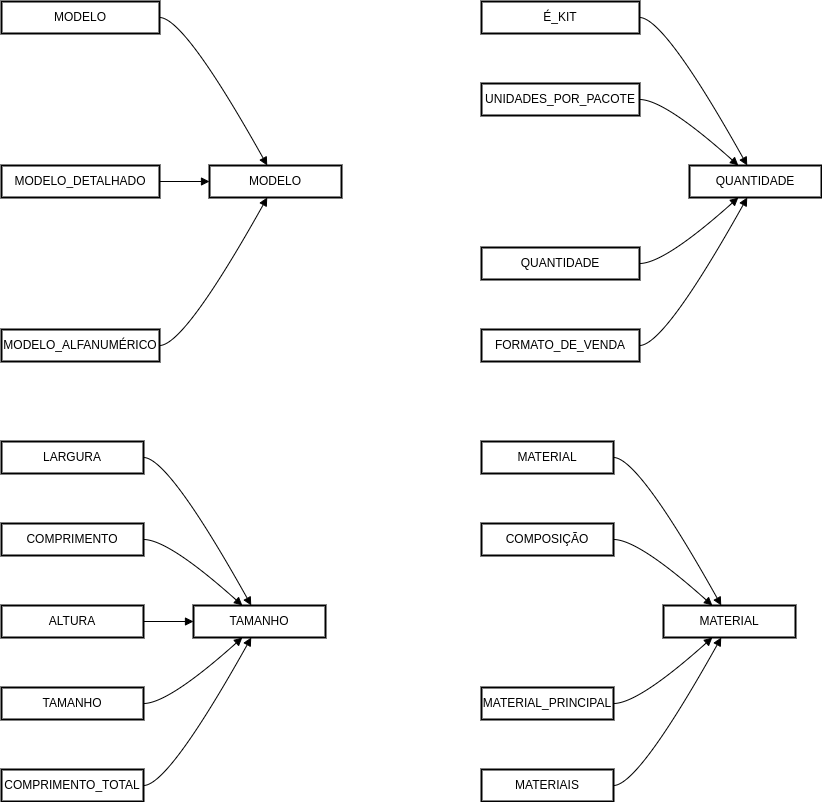
\includegraphics[width=14cm]{figuras/aglutinacao_de_classes_pt.png}
        \caption{Ao início de cada seta, as classes originais que compunham a base de dados com 40 classes. Ao final de cada seta, as classes resultantes da aglutinação, que passaram a compor a base de dados com 28 classes.}
        \label{fig:aglutinacao_classes}
\end{figure}

% Anotação (rotulagem) manual, iterando pelos exemplos das bases de dados da GoBots e assinalando um atributo para cada pergunta que aparecia

\section{Pré-processamento dos Dados}
\label{pre_processamento_dados}
A etapa de pré-processamento dos dados foi feita de forma diferente a depender da arquitetura de Transformador utilizada. Para a arquitetura que usa o modelo BERT para fazer a classificação, essa etapa foi feita apenas com o Tokenizador do modelo BERTimbau Base\footnote{\url{https://huggingface.co/neuralmind/bert-base-portuguese-cased}}, uma variação do modelo BERT pré-treinada em um grande corpus de dados da Internet escritos em Português do Brasil. Para a arquitetura que usa o modelo DIETClassifier para fazer a classificação, essa etapa foi feita com o Tokenizador do modelo BERTimbau Base ou com o Tokenizador do modelo BERT Multilingual Base\footnote{\url{https://huggingface.co/bert-base-multilingual-cased}}, e também com outros componentes extras, explicados na Subseção \ref{prepro_diet_classifier}. O BERT Multilingual Base é uma versão do BERT original desenvolvida pela \textit{Google} que apresenta suporte a 104 idiomas, incluindo o Português.

As etapas de pré-processamento citadas nesta Seção foram realizadas a partir da execução dos mesmos \textit{scripts} usados para o treinamento dos Algoritmos de Classificação: para a arquitetura que usa o modelo BERT para fazer a classificação, o \textit{script} escrito em \textit{Python} que chama funções da biblioteca \textit{HuggingFace Transformers}\footnote{\url{https://github.com/huggingface/transformers/}}; para a arquitetura que usa o modelo DIETClassifier para fazer a classificação, o \textit{script} de linha de comando \textit{rasa train}, incluso com o \textit{software} RASA\footnote{\url{https://rasa.com/}}.

Os exemplos coletados a partir da base de dados da GoBots já estavam sem sinais de pontuação, uma vez que essa etapa de pré-processamento já foi feita quando esses exemplos foram tratados pelo \textit{software} da empresa.

\subsection{BERT}
\label{prepro_bert}
O Tokenizador do modelo BERTimbau Base funciona dividindo a sentença fornecida como entrada em elementos de um vetor, dividindo palavras específicas em múltiplos \textit{tokens} (\textit{Stemming}), associando um número de identificação único a cada \textit{token}, e acrescentando \textit{tokens} especiais que indicam o início e o fim da sentença. Esse Tokenizador não aplica muitos dos passos da etapa de pré-processamento de dados vistos na Seção \ref{pre-processamento dos dados}, pois possui as seguintes caracerísticas:
\begin{itemize}
    \item \textit{Case sensitivity}: ``esse'' e ``Esse'' são tratados como \textit{tokens} diferentes, por exemplo, o que indica a não aplicação de \textit{lowercasing};
    \item Manutenção de \textit{stopwords}: palavras como ``os'' e ``de'' são consideradas \textit{tokens} válidos, por exemplo;
    \item Manutenção da pontuação e/ou números: o ponto de interrogação, por exemplo, é tratado como um \textit{token} individual;
    \item Não aplicação de \textit{Lemmatization}: ``bom'' e ``melhor'' são \textit{tokens} diferentes, por exemplo.
\end{itemize}

As Figuras \ref{fig:br_tokenizer_code} e \ref{fig:br_tokenizer_output} retratam como funciona o processo de Tokenização a partir do Tokenizador do modelo BERTimbau Base relatado. Na Figura \ref{fig:br_tokenizer_code}, \textit{tokenizer} é o Tokenizador do modelo BERTimbau Base, que foi baixado em linhas de código anteriores. Ao receber uma sentença como entrada, ele retorna um dicionário com as chaves ``input\_ids'', ``token\_type\_ids'' e ``attention\_mask'' (Figura \ref{fig:br_tokenizer_output}). O valor da chave ``input\_ids'' é uma lista de números de identificação únicos, onde cada número representa um \textit{token} e está mapeado internamente à uma representação vetorial daquele \textit{token}. Esse dicionário é o que é efetivamente fornecido como entrada ao algoritmo de classificação em treinamento. Se a função \textit{convert\_ids\_to\_tokens()} é chamada, é possível ver quais \textit{tokens} a lista de números de identificação únicos da chave ``input\_ids'' representa (Figura \ref{fig:br_tokenizer_output}).

\begin{figure}[!ht]
    \centering
    \begin{lstlisting}[style=python]
    encoded_text = tokenizer("Esse item |é| feito de silicone?")
    tokens = tokenizer.convert_ids_to_tokens(encoded_text["input_ids"])

    print(encoded_text)
    print(tokens)
    \end{lstlisting}
    \caption{Código em \textit{Python} que faz uso da biblioteca \textit{HuggingFace Transformers} para aplicar um Tokenizador do modelo BERTimbau Base à uma pergunta de um cliente real.}
    \label{fig:br_tokenizer_code}
\end{figure}

\begin{figure}[!ht]
    \centering
    \begin{verbatim}
    {'input_ids': [101, 3758, 18685, 253, 2160, 125, 7296, 10132, 
    22279, 136, 102], 'token_type_ids': [0, 0, 0, 0, 0, 0, 0, 0, 
    0, 0, 0], 'attention_mask': [1, 1, 1, 1, 1, 1, 1, 1, 1, 1, 1]}
    
    ['[CLS]', 'Esse', 'item', 'é', 'feito', 'de', 'sil', '##icon', 
    '##e', '?', '[SEP]']
    \end{verbatim}
    \caption{Saída do código \textit{Python} da Figura \ref{fig:br_tokenizer_code}, mostrando como a pergunta de um cliente real foi pré-processada pelo Tokenizador do modelo BERTimbau Base.}
    \label{fig:br_tokenizer_output}
\end{figure}

\subsection{DIETClassifier}
\label{prepro_diet_classifier}
Como descrito anteriormente, o uso de componentes extras em conjunto com a arquitetura de Transformador \textit{DIETClassifier} diferencia a sua etapa de pré-processamento dos dados em comparação com a etapa de pré-processamento dos dados usada com o BERT. Os componentes extras estão enunciados a seguir, ordenados do primeiro a ser usado ao último:

\begin{itemize}
    \item uma camada de \textit{WhitespaceTokenizer};
    
    O \textit{WhitespaceTokenizer} é um Tokenizador que separa as palavras nos espaços em branco. Além disso, sinais de pontuação no início ou no fim de palavras são removidos. Acentos são mantidos. 
    
    A Figura \ref{fig:whitespace_tokenizer} retrata como o Tokenizador \textit{WhitespaceTokenizer} funciona. Uma lista de \textit{tokens} foi gerada, e cada \textit{token} representa uma palavra da sentença ``Esse item é feito de silicone?''. O acento agudo em ``é'' foi mantido, mas o ponto de interrogação ao final da sentença foi removido, pois ele está ao final de uma palavra. Um \textit{token} especial, chamado de ``\_\_CLS\_\_'', foi introduzido para indicar o fim da sentença.
    
    \item uma camada de \textit{LanguageModelFeaturizer} (constituída pelo Tokenizador do modelo BERTimbau Base ou pelo Tokenizador do modelo BERT Multilingual Base, a depender do experimento);

    O \textit{LanguageModelFeaturizer} funciona da mesma forma que o Tokenizador descrito na Subseção \ref{prepro_bert}.
    
    \item duas camadas de \textit{CountVectorsFeaturizer}.

    O \textit{CountVectorsFeaturizer} é um componente responsável pela transformação dos \textit{tokens} em representações vetoriais. Ele cria representações vetoriais no formato \textit{bag-of-words} da entrada recebida. Na arquitetura de Transformador que usa o modelo DIETClassifier para fazer a classificação, o componente \textit{CountVectorsFeaturizer} foi usado duas vezes: na primeira vez, representações \textit{bag-of-words} foram feitas a nível de palavras; na segunda vez, representações \textit{bag-of-words} foram feitas a nível de sequências de 1 a 5 caracteres. 
    
    A Figura \ref{fig:rasa_tokenizers} retrata como o \textit{CountVectorsFeaturizer} funciona quando aplicado após uma camada de \textit{WhitespaceTokenizer} e uma camada de \textit{LanguageModelFeaturizer}. 
    
    Na parte central da Figura \ref{fig:rasa_tokenizers}, são mostrados os vetores gerados após a aplicação da primeira camada de \textit{CountVectorsFeaturizer}, sendo o primeiro vetor um vetor de \textit{tokens} e o segundo vetor um vetor que indica a quantidade de vezes que cada \textit{token} aconteceu em cada sentença. Os vetores gerados apresentam grande diferença em relação à lista de \textit{tokens} da Figura \ref{fig:whitespace_tokenizer}. Todos os \textit{tokens} ficaram com letras minúsculas. A palavra ``silicone'' foi dividida em múltiplos \textit{tokens}, por causa do \textit{LanguageModelFeaturizer}. `cls' e `sep' são os \textit{tokens} especiais ``\_\_CLS\_\_'' e ``\_\_SEP\_\_'', usados para indicar o fim de cada sentença e o início de uma sentença nova, respectivamente.

    Na parte inferior da Figura \ref{fig:rasa_tokenizers}, são mostrados os vetores gerados após a aplicação da segunda camada de \textit{CountVectorsFeaturizer}. Os \textit{tokens} apresentados são constituídos de todas as sequências de 5 caracteres possíveis de serem criadas a partir das sentenças fornecidas como entrada. Os símbolos \# representam os \textit{tokens} criados a partir da divisão de uma palavra em múltiplos \textit{tokens} (``silicone'' se tornou ``sil'', ``\#\#icon'', ``\#\#e''). Todos os \textit{tokens} ficaram com letras minúsculas. `[cls]' e `[sep]' são os mesmos \textit{tokens} especiais explicados anteriormente. Os vetores constituídos de 1 e 0 na parte inferior indicam quantas vezes cada sequência de 5 caracteres acontece em cada sentença fornecida como entrada.
    
\end{itemize}

\begin{figure}[!ht]
    \begin{subfigure}{\linewidth}
        \centering
        \begin{lstlisting}[style=python]
        "Esse item |é| feito de silicone?"
        \end{lstlisting}
    \end{subfigure}
    
    \begin{subfigure}{\linewidth}
        \centering
        \begin{verbatim}
        ['Esse', 'item', 'é', 'feito', 'de', 'silicone', '__CLS__']
        \end{verbatim}
    \end{subfigure}
    
    \caption{Exemplo de aplicação do Tokenizador \textit{WhitespaceTokenizer}.}
    \label{fig:whitespace_tokenizer}
\end{figure}

\begin{figure}[!ht]
    \begin{subfigure}{\linewidth}
        \centering
        \begin{lstlisting}[style=python]
        ["Esse item |é| feito de silicone?", 
         "Esse item |é| feito de pl|á|stico?"]
        \end{lstlisting}
        \caption{Sentenças de exemplo fornecidas como entrada aos tokenizadores.}
    \end{subfigure}
    
    \hrulefill
    \\
    
    \begin{subfigure}{\linewidth}
        \centering
        \begin{verbatim}
        ['cls' 'de' 'esse' 'feito' 'icon' 'item' 'plástico' 'sep' 'sil']
        [[1 1 1 1 1 1 0 1 1]
        [1 1 1 1 0 1 1 1 0]]
        \end{verbatim}
        \caption{Representações \textit{bag-of-words} a nível de palavras geradas a partir da aplicação dos tokenizadores sobre as sentenças de exemplo fornecidas como entrada.}
    \end{subfigure}

    \hrulefill
    \\

    \begin{subfigure}{\linewidth}
        \centering
        \begin{verbatim}
        ['##e[s' '##ico' '#e[se' '#icon' '[cls]' '[sep]' ']esse' 'cls]e' 
         'co[se' 'con##' 'deplá' 'desil' 'e[sep' 'eitem' 'eitod' 'eméfe' 
         'eplás' 'esil#' 'essei' 'feito' 'ico[s' 'icon#' 'il##i' 'itemé' 
         'itode' 'l##ic' 'ls]es' 'lásti' 'méfei' 'n##e[' 'o[sep' 'odepl' 
         'odesi' 'on##e' 'plást' 's]ess' 'seite' 'sil##' 'sseit' 'stico' 
         'teméf' 'tico[' 'todep' 'todes' 'ástic' 'éfeit']
        [[1 1 1 1 1 1 1 1 0 1 0 1 1 1 1 1 0 1 1 1 0 1 1 1 1 1 1 0 1 1 0
        0 1 1 0 1 1 1 1 0 1 0 0 1 0 1]
        [0 0 0 0 1 1 1 1 1 0 1 0 0 1 1 1 1 0 1 1 1 0 0 1 1 0 1 1 1 0 1
        1 0 0 1 1 1 0 1 1 1 1 1 0 1 1]]
        \end{verbatim}
        \caption{Representações \textit{bag-of-words} a nível de sequências de 5 caracteres geradas a partir da aplicação dos tokenizadores sobre as sentenças de exemplo fornecidas como entrada.}
    \end{subfigure}

    \caption{Resultado após aplicação dos Tokenizadores \textit{WhitespaceTokenizer}, \textit{LanguageModelFeaturizer} e duas camadas de \textit{CountVectorsFeaturizer} em sequência sobre duas sentenças de exemplo.}
    \label{fig:rasa_tokenizers}
\end{figure}

\section{Treinamento dos Algoritmos de Classificação}
\label{algoritmos_classificacao}
Esta seção descreve o método de treinamento dos dois Algoritmos de Classificação usados: BERT e DIETClassifier. Ambos os Algoritmos de Classificação foram treinados por meio de \textit{fine-tuning}, conceito explicado na Subseção \ref{bert_subsubsection}.

As seções de treinamento foram feitas através da plataforma \textit{Google Colaboratory}, em virtude da disponibilidade gratuita de placas de vídeo dedicadas de alto poder computacional. O acesso a esse recurso tornou possível que cada treinamento levasse no máximo 2 horas de duração.

\subsection{BERT}
\label{des_treinamento_hf}
Ao invés de usar o Transformador BERT original, apresentado em \citeonline{bert}, optou-se por usar o BERTimbau Base, apresentado em \citeonline{bertimbau}. Essa escolha foi feita com base nos resultados de experimentos anteriores de outros projetos da empresa GoBots, nos quais chegou-se à conclusão de que modelos treinados com \textit{tokens} em Português apresentam melhores resultados para aplicações em Português, como é o caso deste trabalho.

Os modelos BERTimbau são definidos pelos seus criadores como ``modelos BERT para Português Brasileiro, treinados usando dados do brWaC, um grande \textit{corpus} de páginas Web'' \cite{bertimbau}. À época, os modelos BERTimbau avançaram o estado-da-arte das abordagens BERT multilíngua e monolíngua. O termo Base se refere ao tamanho do modelo menor, de 12 camadas e 110 milhões de parâmetros. Ambos os modelos foram disponibilizados pelos autores para \textit{download} gratuito em bibliotecas \textit{open-source}.

Todas as etapas que usaram o Algoritmo de Classificação BERTimbau Base, do pré-processamento dos dados à Avaliação dos Classificadores, foram feitas por meio de chamadas às funções da biblioteca \textit{HuggingFace Transformers}, escrita na linguagem \textit{Python}. Por meio dela, é possível definir os hiperparâmetros de treino e efetivamente treinar o Algoritmo de Classificação. Para isso, basta que a base de dados esteja em um formato compatível, como JSON ou CSV.

A biblioteca \textit{HuggingFace Transformers} permite a alteração dos hiperparâmetros de treino, tais como \textit{batch\_size} (a quantidade de exemplos vistos a cada passo de treinamento) e \textit{learning\_rate} (o fator pelo qual os pesos do Algoritmo de Classificação em treinamento são multiplicados durante o processo). Por isso, o BERTimbau Base foi treinado em 2 configurações: 

\begin{itemize}
    \item na primeira, identificada como HF1, com quantidade de exemplos a cada passo = 8 exemplos.
    \item na segunda, identificada como HF2, com quantidade de exemplos a cada passo = 1 exemplo. 
\end{itemize}

Ao alterar o número de exemplos que o Algoritmo de Classificação em treinamento vê a cada passo, aumenta-se o número de passos totais para que ele veja todos os exemplos. Assim, ao ver menos exemplos por vez, o Algoritmo é otimizado mais vezes. Foram feitos 5 treinamentos em cada configuração para buscar validade estatística (ou seja, para desprezar efeitos do acaso nas medidas de avaliação que aquele Algoritmo de Classificação atingiu).

Duas rodadas de experimentos foram feitas com o BERTimbau Base: na primeira, as duas configurações HF1 e HF2 foram treinadas na base de dados rotulada em 40 classes. Na segunda rodada de experimentos, foi escolhida a configuração com o melhor desempenho nas medidas de avaliação da primeira rodada para ser treinada na base de dados rotulada em 28 classes.

\subsection{DIETClassifier}
\label{des_treinamento_rasa}
O outro algoritmo de classificação que foi treinado foi o Transformador DIETClassifier, apresentado em \citeonline{diet_classifier}. Um dos motivos pelo qual ele foi escolhido é por causa da modularidade da sua arquitetura, que permite que sejam usados Tokenizadores de variados métodos de pré-treino, assim como outros componentes, em conjunto com ele. Outro motivo para a escolha é que os autores alegam que o melhor modelo DIETClassifier supera um modelo BERT que passou por \textit{fine-tuning} e ainda é seis vezes mais rápido de se treinar \cite{diet_classifier}.

Todas as etapas que usaram o Algoritmo de Classificação DIETClassifier, do pré-processamento dos dados à Avaliação dos Classificadores, foram feitas por meio do \textit{software} de linha de comando RASA \textit{Open Source}. A instalação\footnote{\url{https://rasa.com/docs/rasa/installation/installing-rasa-open-source}} se dá pelo Gerenciador de Pacotes do \textit{Python}, o PIP. Depois disso, é preciso criar um projeto com o comando \textit{rasa init} e procurar os arquivos recém-criados \textit{data/nlu.yml} e \textit{config.yml}. No primeiro arquivo são inseridos todos os exemplos da base de dados. No segundo arquivo são inseridas as especificações de todos os componentes das etapas de pré-processamento dos dados e de Treinamento dos Algoritmos de Classificação. Após o preenchimento dos dois arquivos, é possível começar o treinamento do DIETClassifier com o comando \textit{rasa train nlu}.


O \textit{software} RASA \textit{Open Source} permite a adição e personalização dos componentes do Transformador que será treinado, tais como o \textit{FallbackClassifier}, que retorna uma classe especial indicando que não foi possível prever com assertividade a qual classe aquele exemplo pertence caso a pontuação \textit{confidence} não tenha atingido um valor mínimo de 0.7. Além disso, existe o parâmetro \textit{constrain\_similarities}, que pode ser aplicado ao Algoritmo de Classificação para que seja executada uma função extra para diminuir a similaridade entre a sentença fornecida como entrada e sentenças de outras classes. O DIETClassifier foi treinado em 3 configurações: 

\begin{itemize}
    \item na primeira, identificada como RASA1, o \textit{LanguageModelFeaturizer} usado foi o BERT Multilingual Base, o componente CountVectorsFeaturizer foi configurado para criar representações \textit{bag-of-words} de sequências de 1 a 4 caracteres, o parâmetro \textit{constrain\_similarities} foi definido como verdadeiro e o componente \textit{FallbackClassifier} foi utilizado;
    \item na segunda, identificada como RASA2, o \textit{LanguageModelFeaturizer} usado foi o BERTimbau Base, o componente CountVectorsFeaturizer foi configurado para criar representações \textit{bag-of-words} de sequências de 3 a 5 caracteres, o parâmetro \textit{constrain\_similarities} foi definido como falso e o componente \textit{FallbackClassifier} não foi utilizado;
    \item na terceira, identificada como RASA3, o \textit{LanguageModelFeaturizer} usado foi o BERTimbau Base, o componente CountVectorsFeaturizer foi configurado para criar representações \textit{bag-of-words} de sequências de 3 a 5 caracteres, o parâmetro \textit{constrain\_similarities} foi definido como verdadeiro e o componente \textit{FallbackClassifier} foi utilizado.
\end{itemize}

Duas rodadas de experimentos foram feitas com o DIETClassifier: na primeira, as três configurações RASA1, RASA2 e RASA3 foram treinadas na base de dados rotulada em 40 classes. Na segunda rodada de experimentos, foi escolhida a configuração com o melhor desempenho nas medidas de avaliação da primeira rodada para ser treinada na base de dados rotulada em 28 classes. Foram feitos
5 treinamentos em cada configuração para buscar validade estatística.

\section{Medidas e Método de Avaliação dos Classificadores}
\label{medidas_metodo_avaliacao_classificadores}
Os testes (e consequentemente, a geração de métricas) foram executados pela biblioteca \textit{HuggingFace Transformers} (no caso do BERTimbau Base) ou através de um comando do \textit{software RASA} (no caso do DIETClassifier). Na biblioteca \textit{HuggingFace Transformers}, basta que seja usado o parâmetro \textit{compute\_metrics=} e seja fornecida a função responsável por calcular as métricas. Além das métricas geradas ao final, a biblioteca \textit{HuggingFace Transformers} calcula métricas preliminares toda vez que todos os exemplos de Treinamento são vistos. Contudo, as métricas preliminares foram descartadas, pois não são importantes para os objetivos deste estudo.  No \textit{software RASA Open Source}, a geração de métricas é feita por padrão, sem a adição de novos parâmetros.

Não foi realizada Validação Cruzada nos experimentos com o BERTimbau como Algoritmo de Classificação. A estratégia empregada foi a separação dos dados de Treino e Teste. Os exemplos de Teste, que compõem 20\% da base de dados total, foram usados para os testes, e não influenciaram nos pesos do algoritmo de classificação em treinamento. Os exemplos de Treino, que compõem 80\% da base de dados total, foram usados para o treinamento. Os experimentos foram feitos desta forma por causa da alta demanda de recursos computacionais para realizar Validação Cruzada em treinamentos de modelos BERT, que aumentaria em 5 vezes o tempo necessário para cada um dos 5 treinamentos para ambas as configurações HF1 e HF2.  Além disso, a biblioteca \textit{HuggingFace Transformers} não apresenta suporte nativo a Validação Cruzada, o que dificulta a implementação.

Foi realizada Validação Cruzada nos experimentos com o DIETClassifier, pelo fato deste Algoritmo de Classificação não demandar tantos recursos computacionais para isso quanto o BERTimbau Base. A base de dados definida no arquivo \textit{data/nlu.yml} foi dividida em 5 partes: a cada treinamento, 4 partes eram definidas como exemplos de Treino, e 1 parte era definida como exemplos de Teste, em um processo iterativo. Após todas as partes terem sido definidas como exemplos de Teste, o Treinamento foi finalizado. As métricas de avaliação daquele Treinamento como um todo eram tomadas a partir da média das métricas de avaliação de cada etapa de Validação Cruzada.

É importante salientar que o uso de dois métodos diferentes de avaliação faz com que as métricas encontradas nos experimentos com o algoritmo de classificação BERTimbau não possam ser comparadas com as métricas encontradas nos experimentos com o algoritmo de classificação DIETClassifier. O principal motivo para não se realizar Validação Cruzada na avaliação dos modelos BERTimbau é o fato de que essa técnica aumenta em cinco vezes o número de treinamentos, o que faria que o tempo total gasto com treinamento e avaliação dos modelos BERTimbau passasse de 30 horas para 150 horas e prejudicaria a conclusão dos experimentos.

Além das métricas Acurácia, Precisão, Revocação e F1-Score, as Matrizes de Confusão, como são um bom recurso para comparar o desempenho dos modelos classe a classe e para enxergar pontos fortes e fracos, também foram geradas. A biblioteca \textit{HuggingFace Transformers} não cria Matrizes de Confusão por padrão. Por isso, quando treinando o Transformador que tem como Algoritmo de Classificação o BERTimbau Base, elas foram produzidas com chamadas aos elementos confusion\_matrix() e ConfusionMatrixDisplay() da biblioteca \textit{sklearn.metrics}\footnote{\url{https://scikit-learn.org/stable/modules/generated/sklearn.metrics.confusion_matrix.html}}. Essas chamadas foram adicionadas à função compute\_metrics(). No \textit{software RASA Open Source}, as Matrizes de Confusão são geradas sem adição de código extra.

As métricas F1, Precisão e Revocação foram ponderadas, ou seja, os valores das métricas dependeram também do número de exemplos daquela classe na base de dados. Essa escolha pela ponderação foi feita porque a base de dados é desbalanceada, com algumas classes tendo mais exemplos do que outras. A ponderação é feita fazendo um somatório da multiplicação entre uma métrica de uma classe pela razão entre o número de exemplos daquela classe e o número de exemplos total, como mostra a Equação \ref{eq_weighted}.

\begin{equation}
\label{eq_weighted}
\text{Métrica\_ponderada} = \sum \text{Métrica}_k \cdot \frac{\text{Quant\_exemplos}_k}{\text{Quant\_exemplos}_{\text{total}}}
\end{equation}

\section{Considerações Finais}
Para o desenvolvimento deste estudo, foram aplicadas diferentes abordagens de Classificação de Texto a um problema prático consistido em definir a qual atributo uma determinada pergunta de um usuário real do Mercado Livre se refere.

Na primeira etapa, 39 atributos importantes foram selecionados para serem as classes para as quais as arquiteturas de Transformadores seriam treinadas. Na segunda etapa, dados não-rotulados foram coletados de diferentes fontes. Na terceira etapa, esses dados foram rotulados com o objetivo de criar uma base de dados rotulada. Essa base de dados consiste de 1419 exemplos. Uma segunda rotulação de exemplos com 28 atributos foi feita para que fossem possíveis novos experimentos.

Em seguida, foram definidas formas diferentes de se realizar o pré-processamento dos dados. Para a arquitetura de Transformador que faz uso do classificador BERTimbau Base, apenas o Tokenizador desse classificador foi utilizado. No entanto, para a arquitetura de Transformador que faz uso do classificador DIETClassifier, outros componentes como o \textit{WhitespaceTokenizer} e o \textit{CountVectorsFeaturizer} também foram testados em conjunto com o Tokenizador do BERT Multilingual Base e o Tokenizador do BERTimbau Base.

Finalmente, foi feito o treinamento: 2 configurações diferentes de Transformadores com BERTimbau Base e 3 configurações diferentes de Transformadores com DIETClassifier foram treinadas, 5 vezes cada para que os resultados tenham validade estatística. As configurações com as melhores métricas passaram por uma nova rodada de experimentos sendo treinadas na base de dados com 28 classes. O cálculo de métricas como Acurácia, Precisão, Revocação e F1-Score, assim como a elaboração de Matrizes de Confusão, foi adicionado ao código que faz o treinamento para que fosse possível comparar os modelos treinados.

%TCC:
%TCC:
%TCC:
%TCC: